\section{Comparison with \pathcasemaw Web Interface}
\label{sect:maw_comparison}

\subsection{Features}
\label{sect:maw_comparison_features}

Table \ref{fig:maw_comparison_table} shows a comparison of relevant features
from the online and iPad versions of the \pathcasemaw analysis tools. The
similarities and differences are elaborated here.

\begin{table}[ht!]
\centering
\begin{tabular}{ | p{3in} | l | l | }
    \hline
                        & Online    & iPad \\ \hline

    Molecule and reaction visualization
                        & Yes       & Yes \\ \hline

    SMDA data entry     & Yes       & Yes \\ \hline

    SMDA visualization  & Yes       & Yes \\ \hline

    Lists of reactions, connected pathways, and pathway-related queries in
    tabular form
                        & Yes       & No \\ \hline

    Moving nodes to rearrange the layout
                        & Yes       & No \\ \hline

    Dynamic layout when no frozen layout is present
                        & Yes       & No \\ \hline

    Dynamic layout when no frozen layout is present
                        & Yes       & No \\ \hline

    Highlight differences between SMDA result graphs
                        & No        & Yes \\ \hline
\end{tabular}
    \caption{Functional differences between the online \pathcasemaw pathway
    visualizer and the \mawapp visualizer}
    \label{fig:maw_comparison_table}
\end{table}

The online and iPad-based \pathcasemaw tools supply similar functionality, but
differ for a few reasons. One is the purpose in building the tool. The online
tools are a comprehensive implementation of all \pathcasemaw functionality. The
iPad tools were developed more quickly and only implement the essential
functionality in order to demonstrate the possibility of additional features in
the future. This difference in purpose is responsible for \mawappp lack of
tables of pathways and reactions alongside visualizations, and \mawappp lack of
database queries.

Another source of differing functionality is the technical limitations of the
iPad. iOS applications may only be implemented in C, Objective-C, C++, and a
limited set of scripting languages. Most existing \pathcasemaw code is in C\#
and Java, languages that cannot be used in an iOS application. This limitation
is the main reason that \mawapp cannot generate dynamic layouts; \pathcasemaw
implements dynamic layouts in the Java applet.

User interaction differences force further departures from the interfaces of the
online tools. The web site is able to display an area more than 1024 pixels wide
and of arbitrary height. It may make use of a physical keyboard and small
pointing targets. The iPad, on the other hand, limits the screen to 1024x768
pixels, provides no physical keyboard, and requires that all pointing targets
be large enough to support a pointer as large as a human finger.

\begin{figure}[htb]
    \center{
        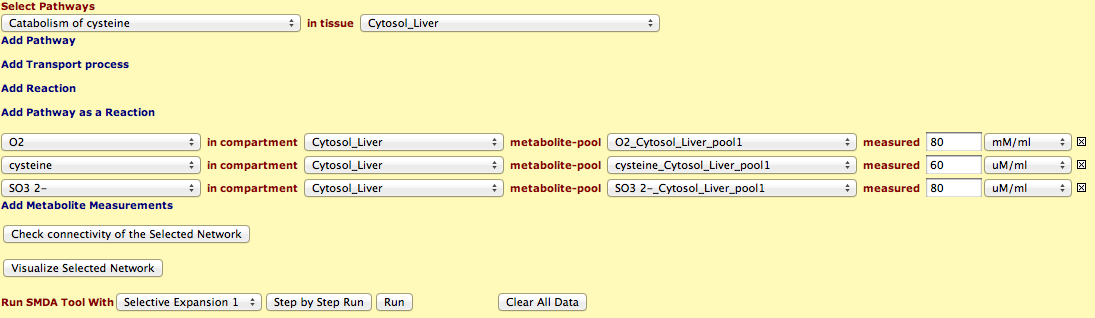
\includegraphics[width=\textwidth]{smda/figures/screenshot_smda_input}}
    \caption{\label{fig:smda_input_online} Online version of SMDA input
    interface}
\end{figure}

To deal with decreased screen space, \mawapp displays less information per
screen. A prime example of this is the SMDA data entry interface. The online
version (see figure \ref{fig:smda_input_online}) mixes the interface for viewing
the entire observation with the interface for entering new data for the
observation, requiring a wide screen to accommodate all fields.

The only functional difference that does not arise from one of these sources is
the addition of green highlights to parts of the SMDA result graphs that change
when the currently displayed result graph is changed. (See figure
\ref{fig:smda_results_highlight}.) This was a change initially introduced to
assist debugging, but it proved useful enough that it remains in the final
version. This feature may be added to the online tool in the future.
